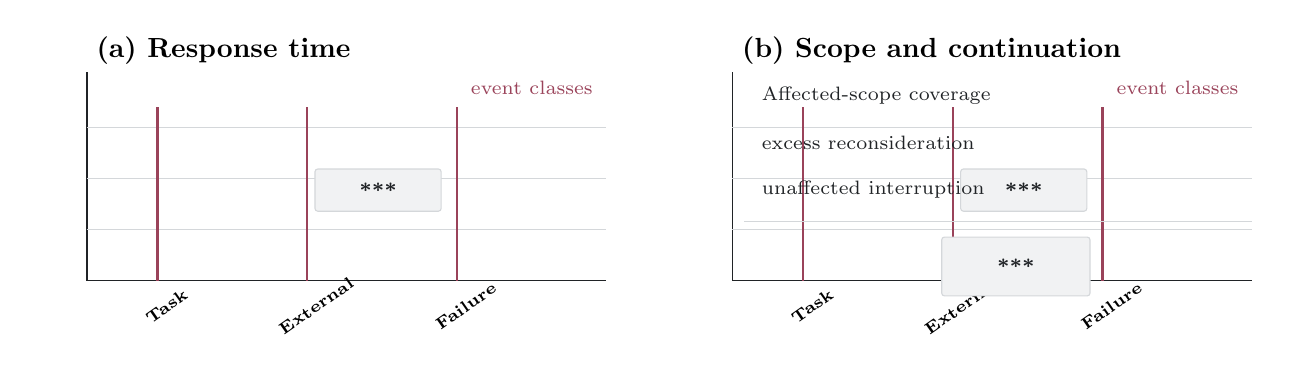
\begin{tikzpicture}[x=1cm,y=1cm,font=\rmfamily\fontsize{7.5}{8.3}\selectfont]
  \definecolor{grid}{HTML}{D4D7DA}
  \definecolor{ink}{HTML}{202326}
  \definecolor{event}{HTML}{9A435A}
  \definecolor{placeholder}{HTML}{F1F2F3}
  \foreach \x/\paneltitle in {0/{(a) Response time},8.2/{(b) Scope and continuation}}{
    \begin{scope}[shift={(\x,0)}]
      \draw[ink,line width=0.6pt] (0.75,0.60) -- (7.35,0.60);
      \draw[ink,line width=0.6pt] (0.75,0.60) -- (0.75,3.25);
      \foreach \yy in {1.25,1.90,2.55}{\draw[grid,line width=0.35pt] (0.75,\yy)--(7.35,\yy);}
      \node[anchor=west,font=\bfseries] at (0.75,3.52) {\paneltitle};
      \foreach \xx/\lab in {1.65/Task,3.55/External,5.45/Failure}{
        \draw[event,line width=0.8pt] (\xx,0.60)--(\xx,2.80);
        \node[anchor=north,font=\bfseries\fontsize{6.5}{7}\selectfont,
          rotate=35] at (\xx,0.44) {\lab};
      }
      \node[draw=grid,fill=placeholder,rounded corners=1pt,text=ink,
            inner xsep=16pt,inner ysep=5pt] at (4.45,1.75) {\bfseries ***};
      \node[anchor=east,text=event] at (7.30,3.05) {event classes};
    \end{scope}
  }
  \begin{scope}[shift={(8.2,0)}]
    \node[anchor=west,text=ink] at (1.0,2.95) {Affected-scope coverage};
    \node[anchor=west,text=ink] at (1.0,2.35) {excess reconsideration};
    \node[anchor=west,text=ink] at (1.0,1.75) {unaffected interruption};
    \draw[grid,line width=0.35pt] (0.9,1.35)--(7.35,1.35);
    \node[draw=grid,fill=placeholder,rounded corners=1pt,text=ink,
          inner xsep=20pt,inner ysep=8pt] at (4.35,0.78) {\bfseries ***};
  \end{scope}
  \path[use as bounding box] (0.0,0.0) rectangle (15.95,3.75);
\end{tikzpicture}
